\documentclass[12pt]{article}

\usepackage[utf8]{inputenc}
\usepackage[T1]{fontenc}
\usepackage[polish,provide=*]{babel}
\usepackage{lmodern}
\usepackage{amsmath}
\usepackage{latexsym,amsfonts,amssymb,amsthm,amsmath}
\usepackage{enumitem}
\usepackage{float}
\usepackage{hyperref}
\usepackage{graphicx}
\usepackage{subcaption}
\usepackage{booktabs}
\graphicspath{{./images/}}

\setlength{\parindent}{0in}
\setlength{\oddsidemargin}{0in}
\setlength{\textwidth}{6.5in}
\setlength{\textheight}{8.8in}
\setlength{\topmargin}{0in}
\setlength{\headheight}{18pt}

\title{}
\author{Kacper Kłos}

\begin{document}

\maketitle

W raporcie analizowaliśmy zachowanie kabla przy bardzo szybkich sygnałach. Wysyłaliśmy sygnały o napięciu 5 V mający 100 ns oraz 10 ns trwa zwiększenie napięcia z 0 do 5 V

\newpage


\section{Wyniki Pomierów}
Wpierw badaliśmy czas potrzebny do odbicia sygnału dla kabla dobrego i złego i impedencji \(75 \, \mathrm{\Omega}\).

\begin{table}[H]
    \centering
    \begin{tabular}{c|cc|cc}
        \toprule
        \textbf{Nr} & \multicolumn{2}{c|}{\textbf{Dobry kabel}} & \multicolumn{2}{c}{\textbf{Zły kabel}} \\
        & $d$ [m] & $t$ [ns] & $d$ [m] & $t$ [ns] \\
        \midrule
        1  & 30  & 154 & 20  & 84 \\
        2  & 60  & 304 & 40  & 164 \\
        3  & 40  & 206 & 40  & 174 \\
        4  & 80  & 406 & 80  & 346 \\
        5  & 65  & 332 & 60  & 264 \\
        6  & 130 & 662 & 120 & 524 \\
        7  & 80  & 404 & 80  & 356 \\
        8  & 160 & 810 & 160 & 708 \\
        9  & --  & --      & 100 & 438 \\
        10 & --  & --      & 200 & 872 \\
        \bottomrule
    \end{tabular}
    \caption{Porównanie pomiarów odległości $d$ i czasu $t$ dla dobrego i uszkodzonego kabla.}
    \label{tab:good_vs_bad_cable}
\end{table}

\begin{figure}[H]
  \centering
  \begin{subfigure}{0.45\textwidth}
    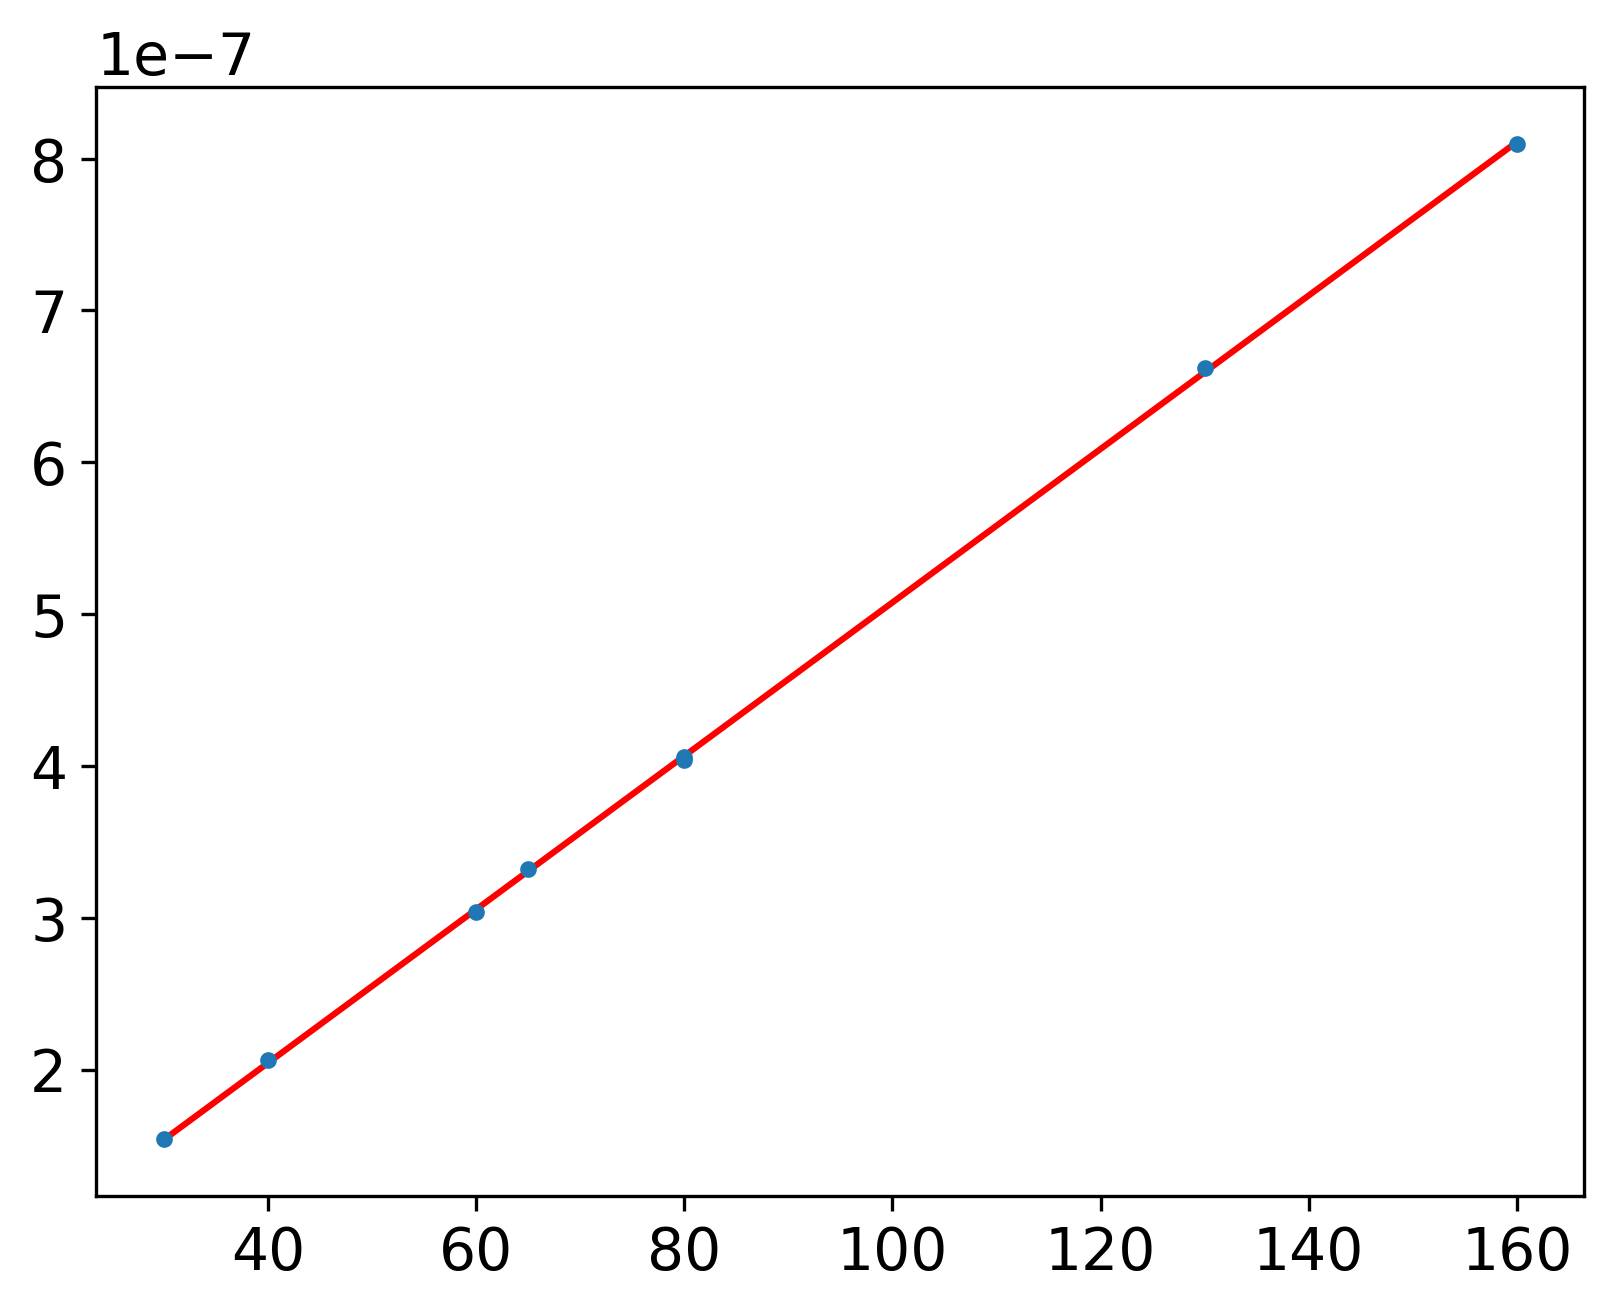
\includegraphics[width=\linewidth]{good_cable_distance}
    \caption{Dobry kabel}
    \label{fig:good_distance}
  \end{subfigure}\hfill
  \begin{subfigure}{0.45\textwidth}
    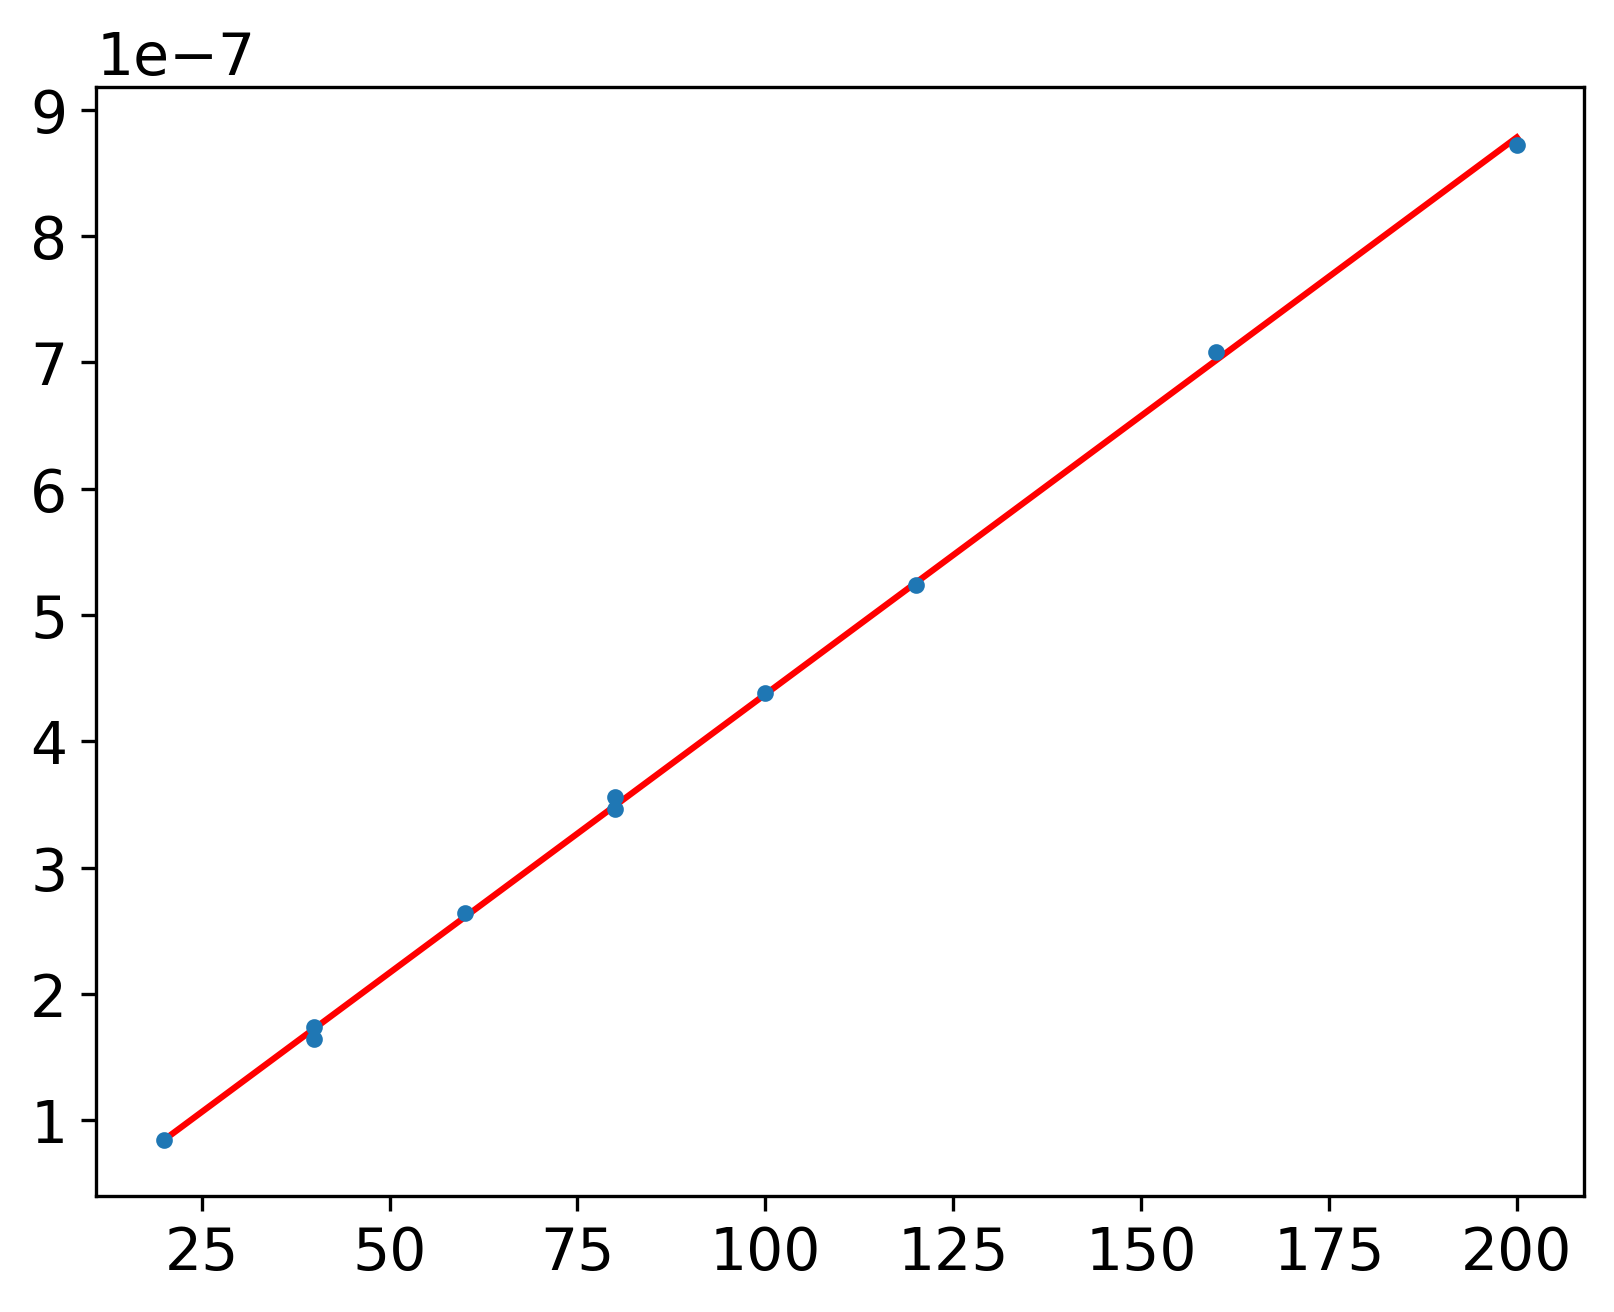
\includegraphics[width=\linewidth]{bad_cable_distance}
    \caption{Zły kabel}
    \label{fig:bad_distance}
  \end{subfigure}
  \caption{Wykres czasu między wysłanym a odebranym sygnałem \(t\) od długości kabla \(d\).}
  \label{fig:distance}
\end{figure}

Następnie mierzymy napięcie odbitego sygnały od oporu podłączonego do końca kabla.

\begin{table}[H]
    \centering
    \begin{tabular}{c|cc|cc}
        \toprule
        \textbf{Nr} & \multicolumn{2}{c|}{\textbf{Dobry kabel}} & \multicolumn{2}{c}{\textbf{Zły kabel}} \\
        & $R$ [$\Omega$] & $U$ [V] & $R$ [$\Omega$] & $U$ [V] \\
        \midrule
        1  & 21{,}242  & -1{,}200 & 5{,}949  & -1{,}760 \\
        2  & 67{,}889  & -0{,}080 & 21{,}741 & -1{,}160 \\
        3  & 51{,}489  & -0{,}400 & 50{,}467 & -0{,}440 \\
        4  & 98{,}712  & 0{,}320  & 73{,}712 & -0{,}040 \\
        5  & 154{,}450 & 0{,}800  & 99{,}180 & 0{,}280 \\
        6  & 229{,}724 & 1{,}080  & 154{,}913 & 0{,}680 \\
        7  & 346{,}970 & 1{,}400  & 228{,}870 & 0{,}960 \\
        8  & 426{,}380 & 1{,}600  & 324{,}130 & 1{,}200 \\
        9  & 502{,}590 & 1{,}680  & 423{,}340 & 1{,}480 \\
        10 & 5{,}985   & -1{,}920 & 502{,}510 & 1{,}520 \\
        \bottomrule
    \end{tabular}
    \caption{Porównanie pomiarów rezystancji $R$ i napięcia $U$ dla dobrego i uszkodzonego kabla.}
    \label{tab:good_vs_bad_cable_voltage}
\end{table}

\begin{figure}[H]
  \centering
  \begin{subfigure}{0.45\textwidth}
    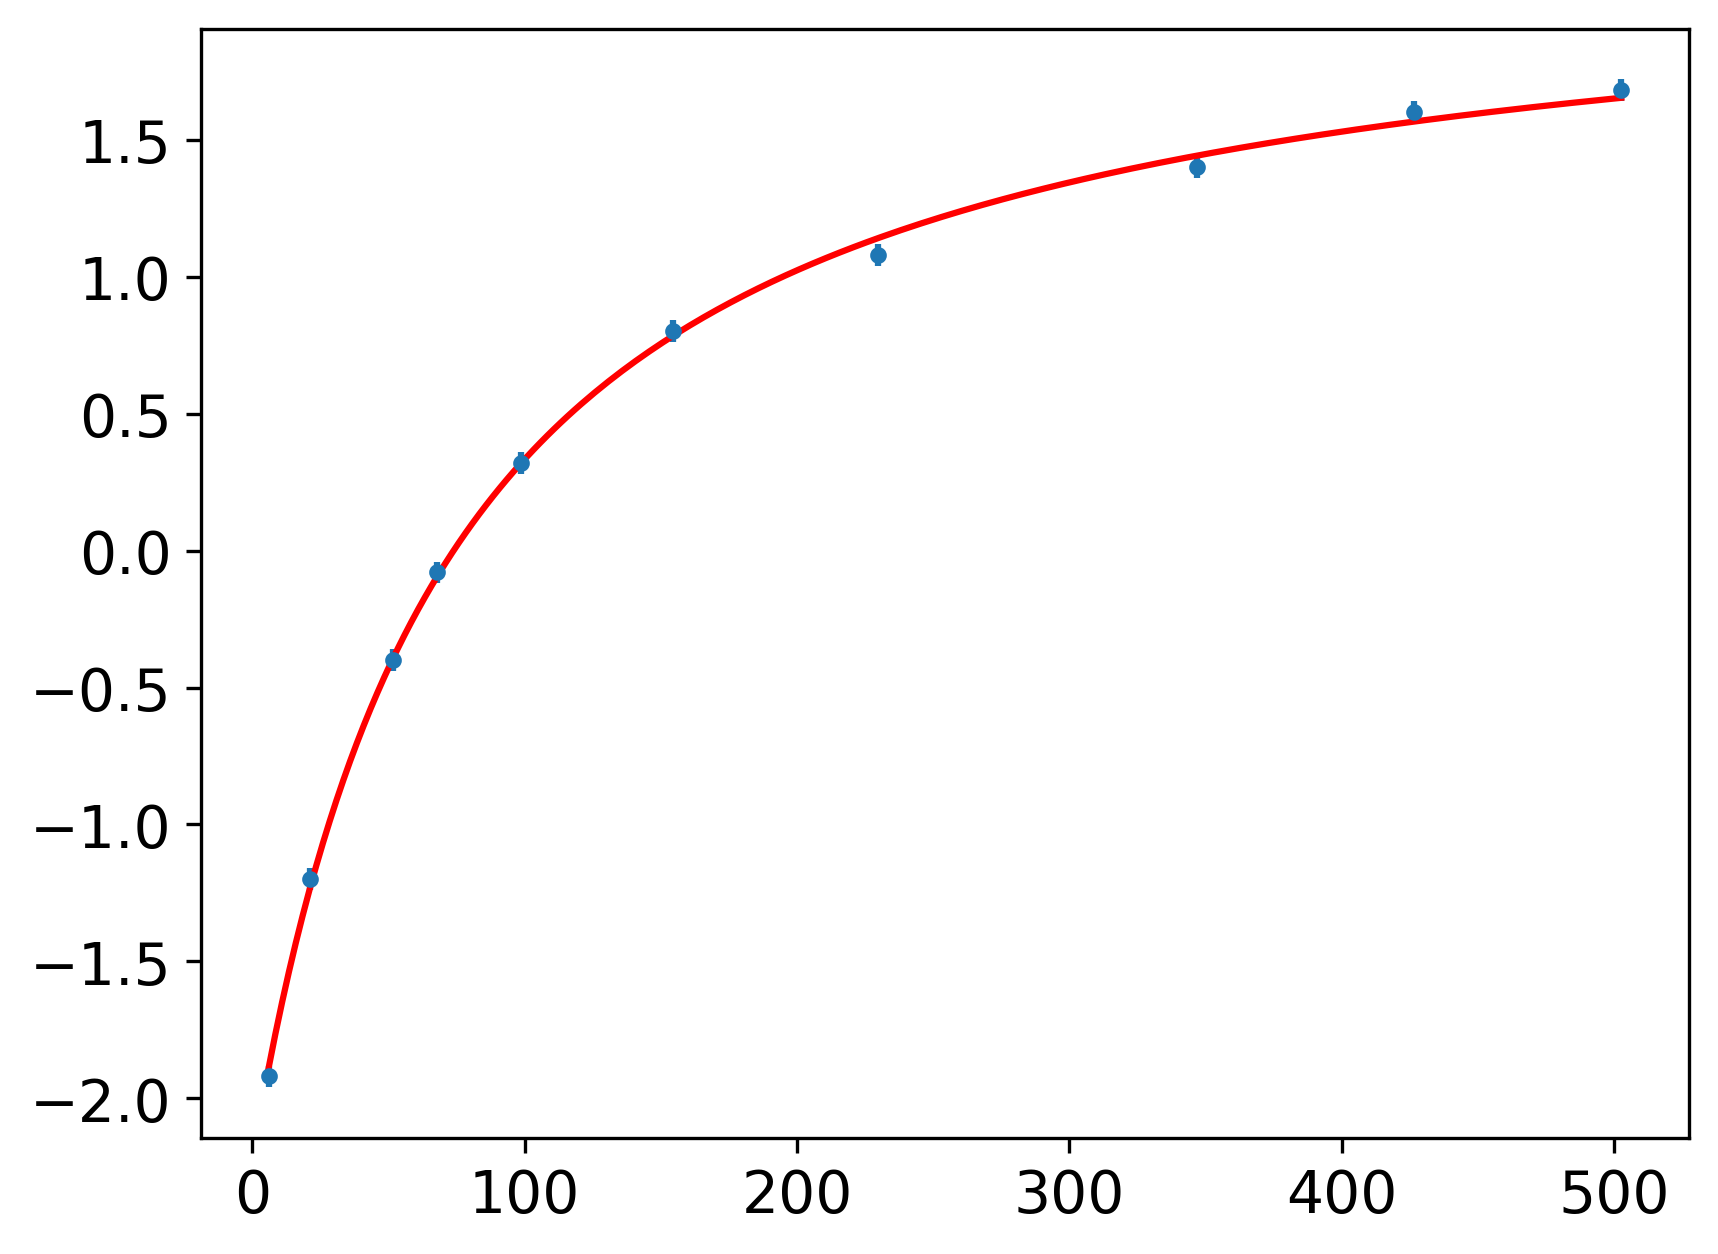
\includegraphics[width=\linewidth]{good_cable_voltage}
    \caption{Dobry kabel}
    \label{fig:good_distance}
  \end{subfigure}\hfill
  \begin{subfigure}{0.45\textwidth}
    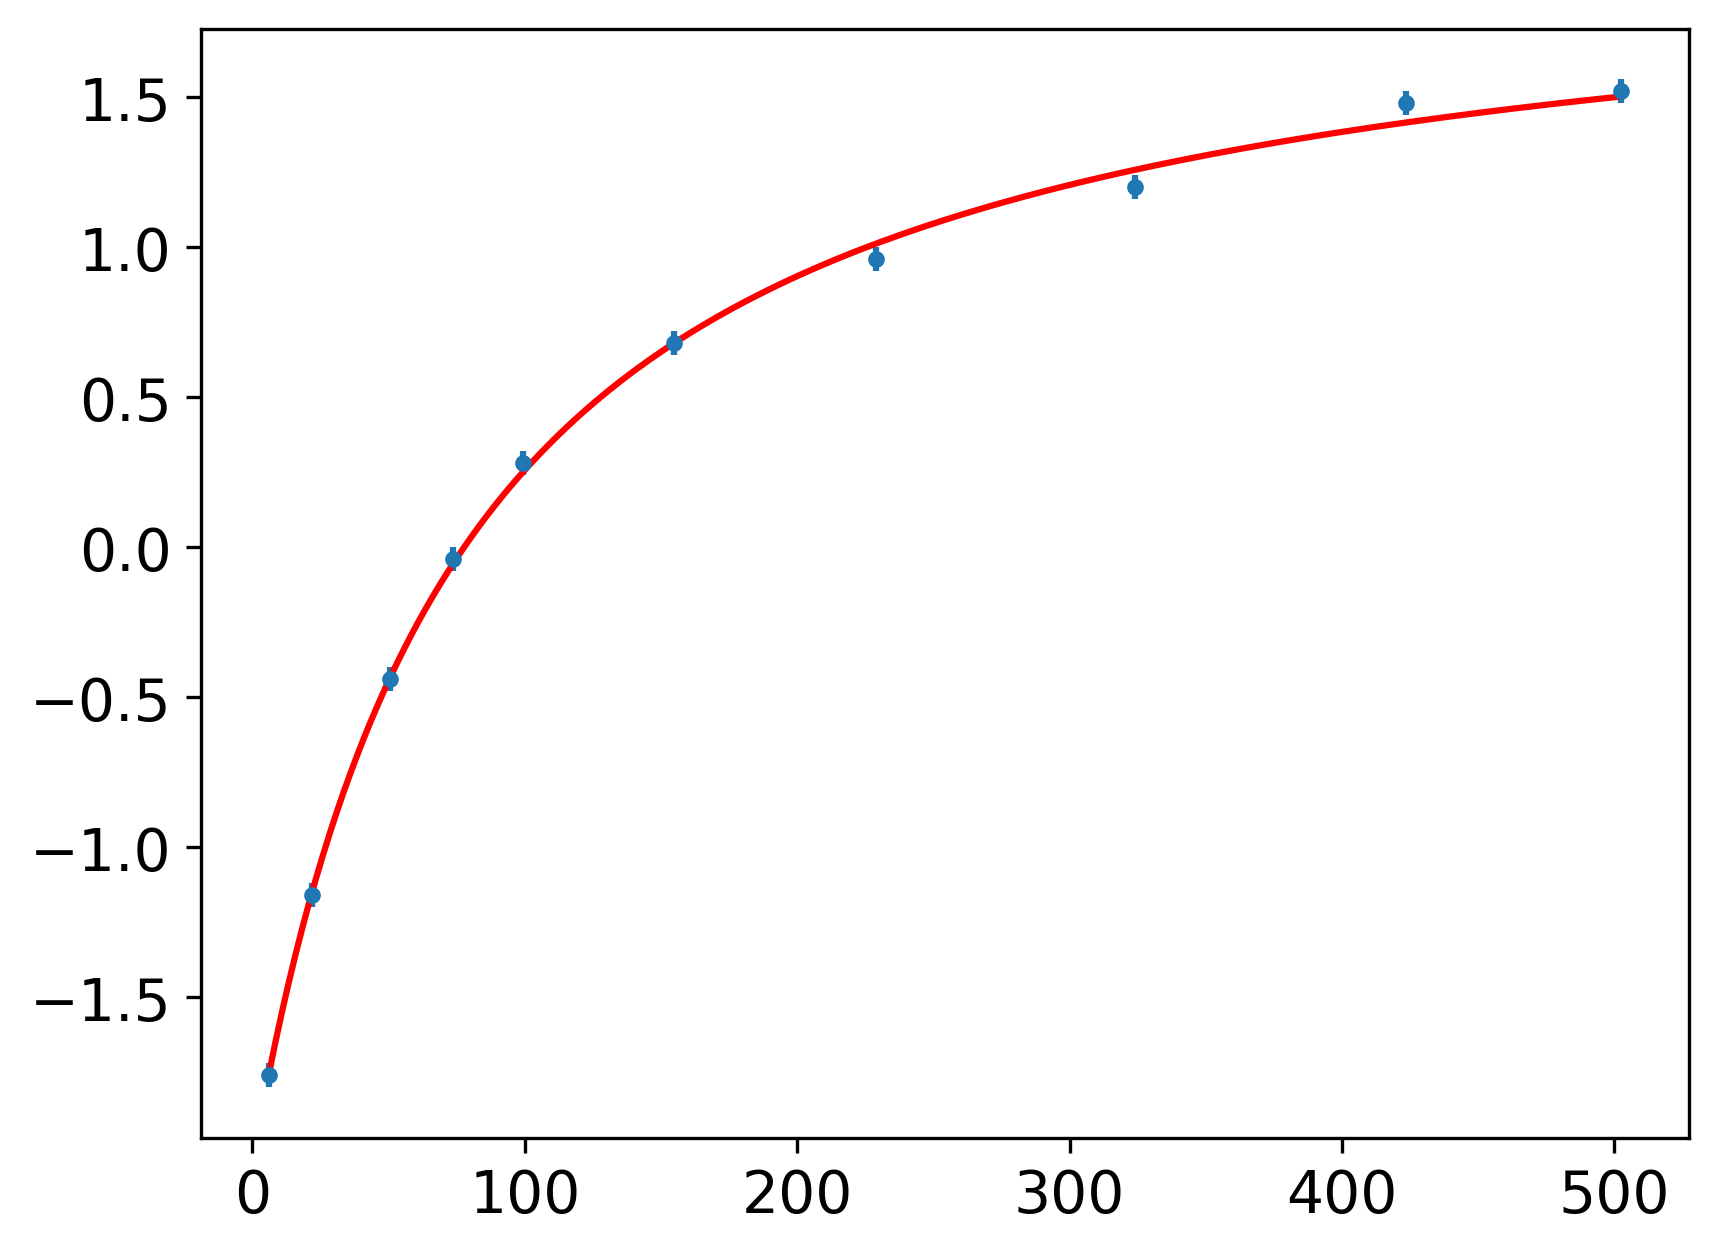
\includegraphics[width=\linewidth]{bad_cable_voltage}
    \caption{Zły kabel}
    \label{fig:bad_distance}
  \end{subfigure}
  \caption{Wykres napięcia odbitego sygnału \(U\) od oporu na końcu przewodu \(R\)}
  \label{fig:distance}
\end{figure}

\section{Podsumowanie}




\end{document}
